\documentclass[aspectratio=169,11pt]{beamer}

% =========================================================
% Presentacion Beamer
% Tema: funciones iteradas, bifurcacion logistica y map tent
% Enfoque: curso de Modelos Matematicos I
% =========================================================

\usepackage[utf8]{inputenc}
\usepackage[T1]{fontenc}
\usepackage{lmodern}
\usepackage[spanish,es-nodecimaldot]{babel}
\usepackage{amsmath,amssymb,mathtools}
\usepackage{tikz}
\usepackage{booktabs}
\usepackage{listings}

\usetheme{Madrid}
\usecolortheme{default}
\setbeamertemplate{navigation symbols}{}
\setbeamertemplate{footline}[frame number]

\lstset{
    language=Python,
    basicstyle=\ttfamily\tiny,
    keywordstyle=\color{blue!70!black},
    commentstyle=\color{green!45!black}\itshape,
    stringstyle=\color{orange!80!black},
    showstringspaces=false,
    columns=fullflexible,
    aboveskip=0pt,
    belowskip=0pt,
}
\newsavebox{\codebox}

\newcommand{\Fmu}{F_\mu}
\newcommand{\Tdos}{T_2}
\newcommand{\orb}{\mathcal O^+}

\title[Funciones iteradas y bifurcaci\'on]{Funciones iteradas, bifurcaci\'on log\'istica y map tent}
\subtitle{Una lectura desde Modelos Matem\'aticos I}
\author{Alejandro Cruz L\'opez \\
        Sergio Antonio Hernández Peralta}
\date{}

\begin{document}

% 1
\begin{frame}
    \titlepage
    \vspace{-0.4cm}
    \begin{center}
        \small Objetivo: explicar c\'omo una regla simple de evoluci\'on puede producir equilibrio, oscilaciones, bifurcaciones y caos.
    \end{center}
\end{frame}

% 2
\begin{frame}{Puente con el curso}
    \begin{itemize}
        \item En el curso se estudiaron modelos en tiempo continuo:
        \[
        \frac{dy}{dt}=f(y).
        \]
        \item Ahora consideramos modelos en tiempo discreto:
        \[
        x_{n+1}=f(x_n).
        \]
        \item La pregunta sigue siendo cualitativa: \textbf{\textquestiondown{}qu\'e ocurre a largo plazo?}
    \end{itemize}
\end{frame}

% 3
\begin{frame}{Funci\'on como regla de evoluci\'on}
    \begin{itemize}
        \item Una funci\'on $f:I\to I$ actualiza estados.
        \item Si $x_n$ es el estado actual, entonces:
        \[
        x_{n+1}=f(x_n).
        \]
        \item La funci\'on se convierte en un modelo din\'amico cuando se aplica repetidamente.
    \end{itemize}
\end{frame}

% 4
\begin{frame}{Iteraci\'on}
    \begin{itemize}
        \item Segunda iteraci\'on:
        \[
        f^2=f\circ f.
        \]
        \item Tercera iteraci\'on:
        \[
        f^3=f\circ f\circ f.
        \]
        \item Trayectoria discreta:
        \[
        x_0,\quad f(x_0),\quad f^2(x_0),\quad f^3(x_0),\ldots
        \]
    \end{itemize}
\end{frame}

% 5
\begin{frame}{\'Orbitas}
    \begin{itemize}
        \item La \textit{\'orbita positiva} de $x$ es:
        \[
        \orb(x)=\{x,f(x),f^2(x),\ldots\}.
        \]
        \item En modelos discretos, la \textit{\'orbita} reemplaza a la curva soluci\'on continua.
        \item Puede converger, volverse peri\'odica o comportarse irregularmente.
    \end{itemize}
\end{frame}

% 6
\begin{frame}{Equilibrio continuo vs punto fijo discreto}
    \begin{columns}
        \column{0.48\textwidth}
        \textbf{Tiempo continuo}
        \[
        y'=f(y)
        \]
        \[
        f(y^*)=0
        \]
        \begin{center}
        equilibrio
        \end{center}
        \column{0.48\textwidth}
        \textbf{Tiempo discreto}
        \[
        x_{n+1}=f(x_n)
        \]
        \[
        f(p)=p
        \]
        \begin{center}
        punto fijo
        \end{center}
    \end{columns}
\end{frame}

% 7
\begin{frame}{Puntos fijos}
    \begin{itemize}
        \item Un punto fijo satisface:
        \[
        f(p)=p.
        \]
        \item Interpretaci\'on: si el sistema llega a $p$, permanece en $p$.
        \item Gr\'aficamente: intersecci\'on entre $y=f(x)$ y $y=x$.
    \end{itemize}
    \begin{center}
    \begin{tikzpicture}[scale=0.75]
        \draw[->] (-0.2,0) -- (4.2,0) node[right] {$x$};
        \draw[->] (0,-0.2) -- (0,3.2) node[above] {$y$};
        \draw[thick] (0,0) -- (3.2,3.2) node[right] {$y=x$};
        \draw[thick,blue,domain=0:3.4,smooth] plot (\x,{1.8+0.55*(\x-1.8)+0.18*sin(120*(\x-1.8))});
        \filldraw[red] (1.8,1.8) circle (2pt) node[below right] {$p$};
    \end{tikzpicture}
    \end{center}
\end{frame}

% 8
\begin{frame}{Estabilidad de puntos fijos}
    \begin{itemize}
        \item En EDO escalar:
        \[
        f'(y^*)<0 \Rightarrow y^* \text{ estable}, \qquad
        f'(y^*)>0 \Rightarrow y^* \text{ inestable}.
        \]
        \item En mapas discretos:
        \[
        |f'(p)|<1 \Rightarrow p \text{ atractor}, \qquad
        |f'(p)|>1 \Rightarrow p \text{ repulsor}.
        \]
        \item El caso $|f'(p)|=1$ es cr\'itico.
    \end{itemize}
\end{frame}

% 9
\begin{frame}{Linealizaci\'on}
    \begin{itemize}
        \item Cerca de un punto fijo $p$:
        \[
        f(x)\approx f(p)+f'(p)(x-p).
        \]
        \item Como $f(p)=p$:
        \[
        x_{n+1}-p\approx f'(p)(x_n-p).
        \]
        \item La derivada mide si las perturbaciones se contraen o se amplifican.
    \end{itemize}
\end{frame}

% 10
\begin{frame}{Modelo log\'istico continuo}
    \begin{itemize}
        \item Modelo poblacional visto en el curso:
        \[
        \frac{dN}{dt}=rN\left(1-\frac{N}{K}\right),\qquad r,K>0.
        \]
        \item Equilibrios:
        \[
        N=0,\qquad N=K.
        \]
        \item $K$ representa la capacidad de carga del entorno.
    \end{itemize}
\end{frame}

% 11
\begin{frame}{Normalizaci\'on del log\'istico}
    \begin{itemize}
        \item Variables adimensionales:
        \[
        u=\frac{N}{K},\qquad \tau=rt.
        \]
        \item Forma normalizada:
        \[
        \frac{du}{d\tau}=u(1-u).
        \]
        \item La normalizaci\'on elimina par\'ametros y conserva la estructura din\'amica.
    \end{itemize}
\end{frame}

% 12
\begin{frame}{Log\'istico discreto}
    \begin{itemize}
        \item Mapa log\'istico:
        \[
        \Fmu(x)=\mu x(1-x).
        \]
        \item Modelo discreto:
        \[
        x_{n+1}=\Fmu(x_n).
        \]
        \item El par\'ametro $\mu$ controla el comportamiento de las \textit{\'orbitas}.
    \end{itemize}
\end{frame}

% 13
\begin{frame}{Puntos fijos del log\'istico discreto}
    \begin{itemize}
        \item Se resuelve:
        \[
        \Fmu(x)=x.
        \]
        \item Entonces:
        \[
        \mu x(1-x)=x.
        \]
        \item Puntos fijos:
        \[
        x=0,\qquad p_\mu=\frac{\mu-1}{\mu}.
        \]
    \end{itemize}
\end{frame}

% 14
\begin{frame}{Estabilidad del log\'istico discreto}
    \begin{itemize}
        \item Derivada:
        \[
        \Fmu'(x)=\mu(1-2x).
        \]
        \item En $x=0$:
        \[
        \Fmu'(0)=\mu.
        \]
        \item En $p_\mu=(\mu-1)/\mu$:
        \[
        \Fmu'(p_\mu)=2-\mu.
        \]
        \item Por tanto, $p_\mu$ es estable si $1<\mu<3$.
    \end{itemize}
\end{frame}

% 15
\begin{frame}{Bifurcaci\'on}
    \begin{itemize}
        \item En el curso: una bifurcaci\'on cambia el n\'umero o la estabilidad de equilibrios.
        \item En mapas: tambi\'en pueden cambiar los ciclos peri\'odicos.
        \item En $\mu=3$:
        \[
        \Fmu'(p_\mu)=-1.
        \]
        \item El punto fijo pierde estabilidad y aparece una \textit{\'orbita} de periodo $2$.
    \end{itemize}
\end{frame}

% 16
\begin{frame}{Duplicaci\'on de periodo}
    \begin{itemize}
        \item Al aumentar $\mu$, el atractor cambia:
        \[
        1\longrightarrow 2\longrightarrow 4\longrightarrow 8\longrightarrow\cdots
        \]
        \item Primero hay un punto fijo atractor.
        \item Luego aparece un ciclo de periodo $2$.
        \item Despu\'es ciclos de periodo $4$, $8$, $16$, etc.
    \end{itemize}
\end{frame}

% 17
\begin{frame}[fragile]{Diagrama de bifurcaci\'on log\'istico}
    \begin{columns}[c]
        \column{0.56\textwidth}
            \centering
            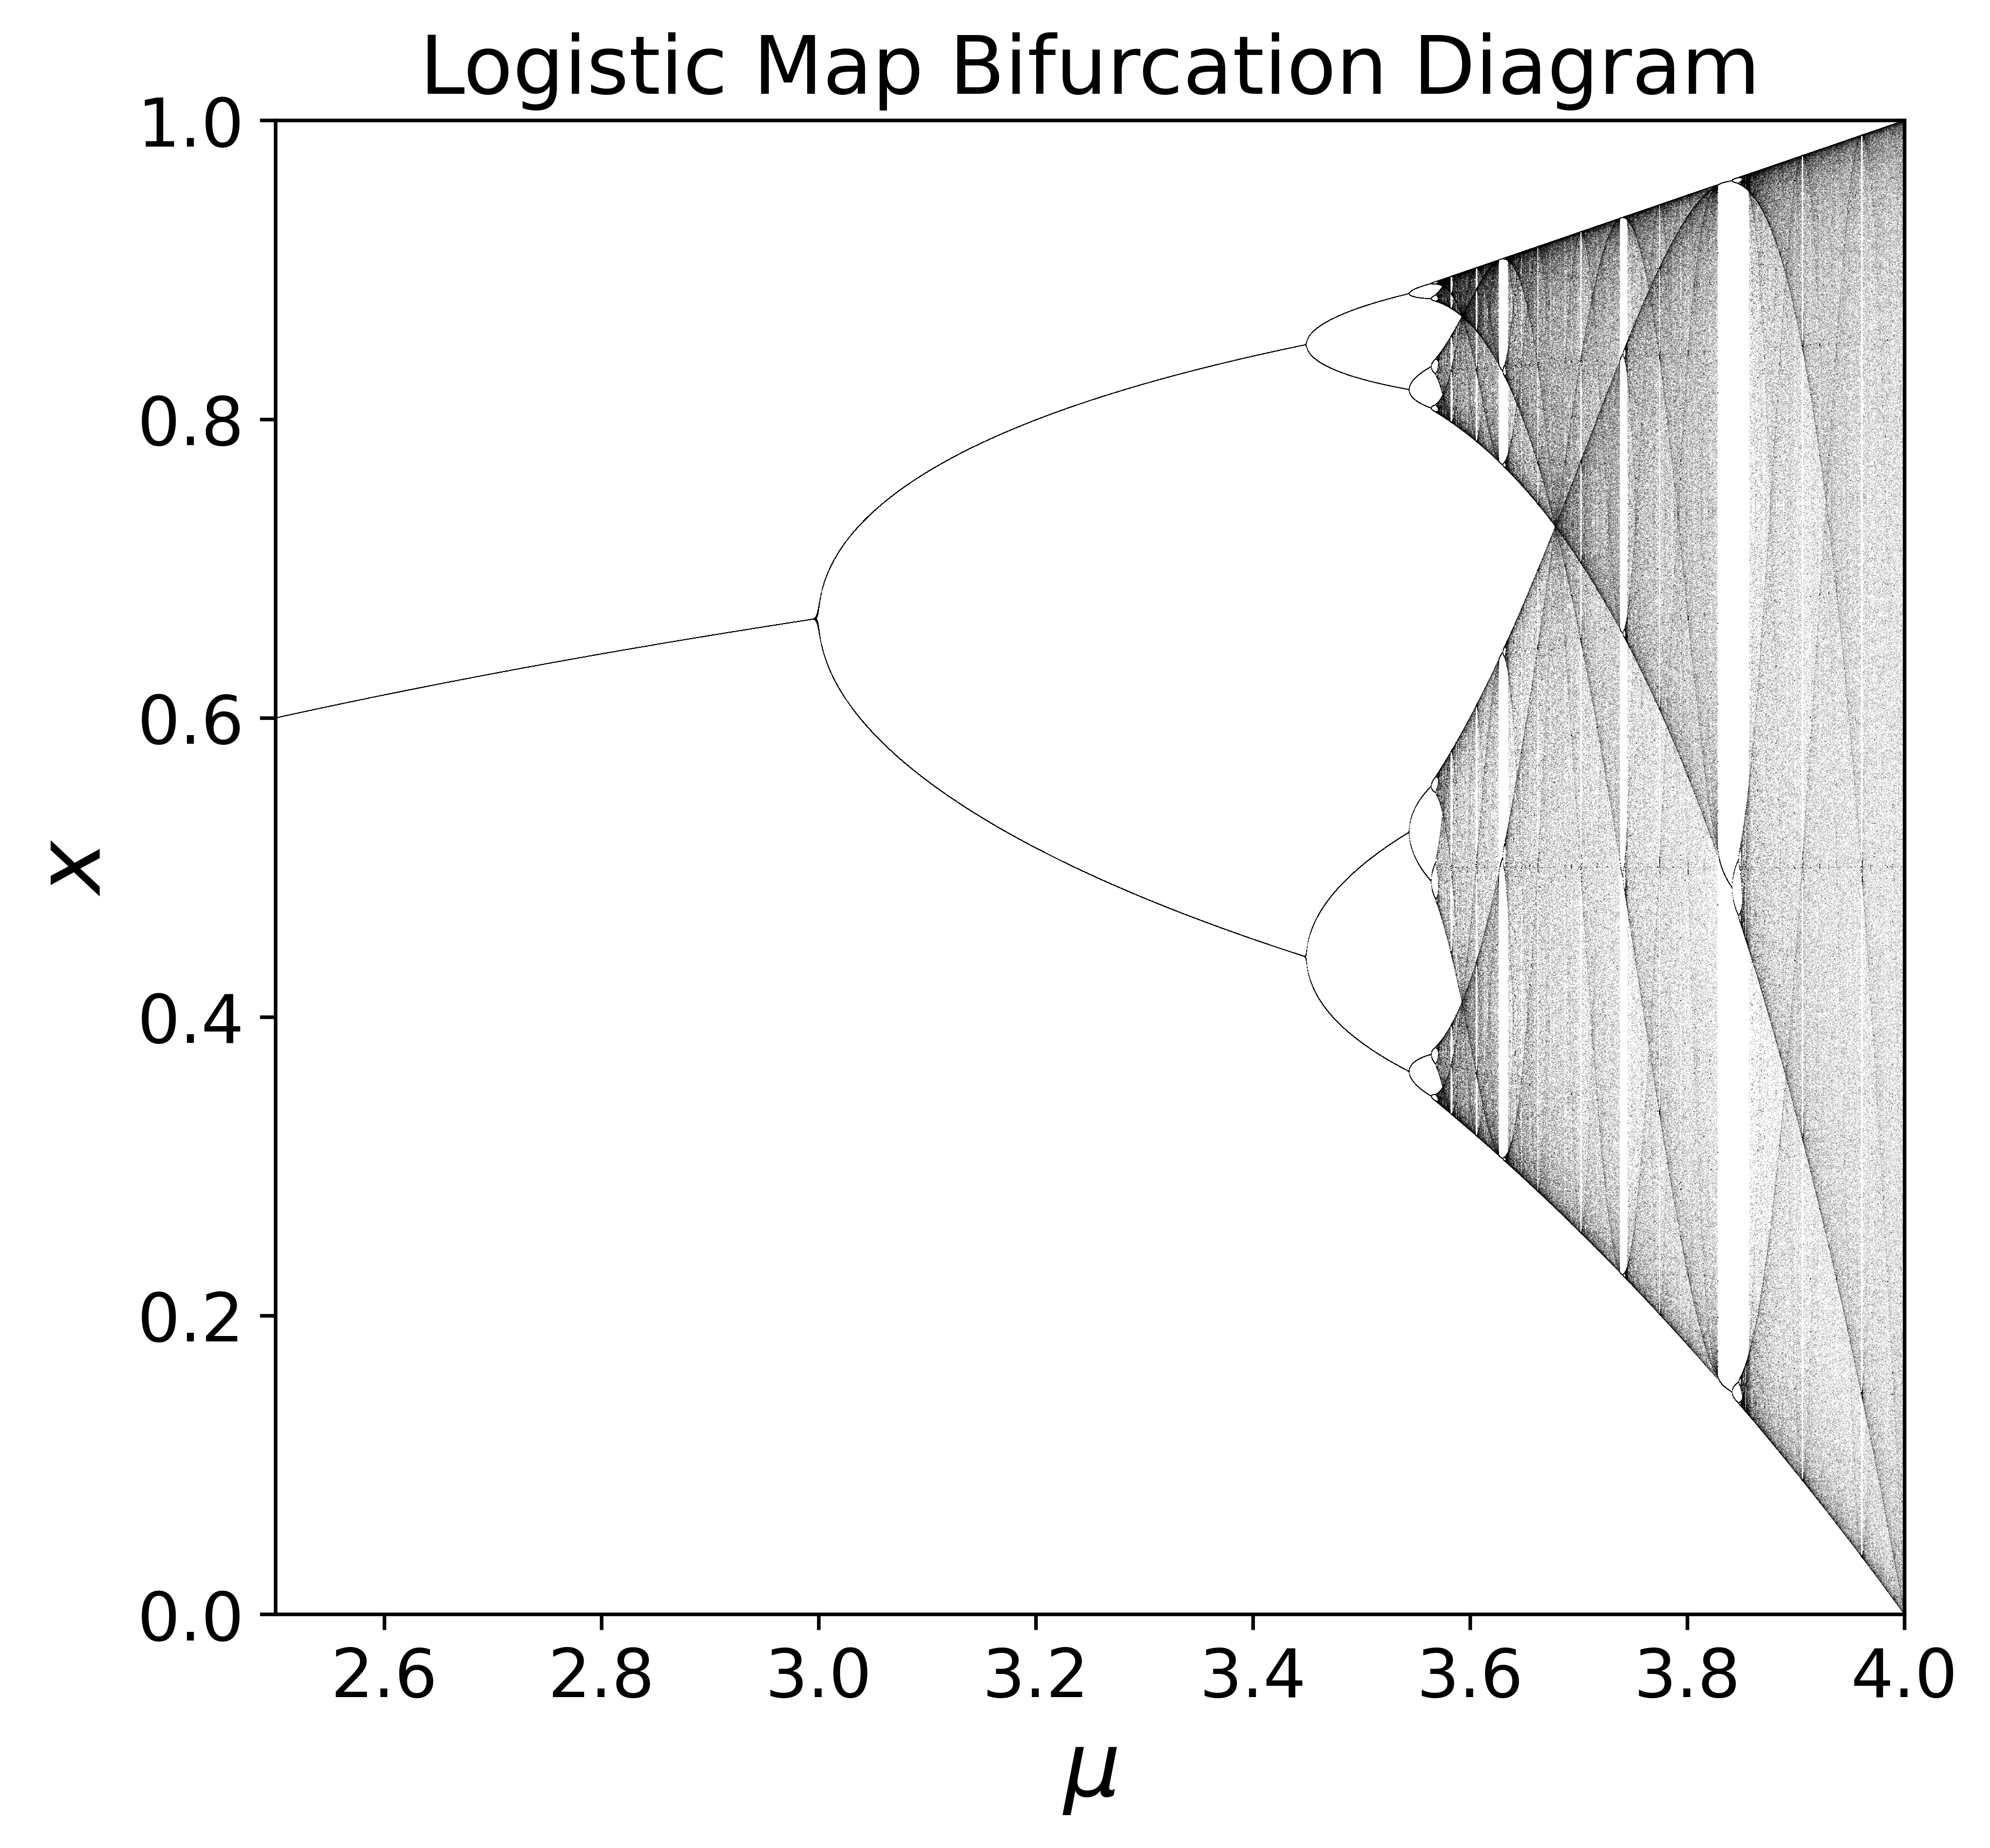
\includegraphics[width=\textwidth]{logistic-map-fig/logistic_map.png}
        \column{0.44\textwidth}
            \lstinputlisting[basicstyle=\ttfamily\fontsize{6.3}{7.0}\selectfont]{logistic-map-fig/logistic_simple.py}
    \end{columns}
\end{frame}

% 18
\begin{frame}{Map tent}
    \begin{itemize}
        \item Definici\'on:
        \[
        \Tdos(x)=
        \begin{cases}
        2x, & 0\leq x\leq \frac12,\\
        2(1-x), & \frac12\leq x\leq 1.
        \end{cases}
        \]
        \item Es lineal por partes.
        \item Tiene forma geom\'etrica de tienda.
    \end{itemize}
\end{frame}

% 18b
\begin{frame}{La funci\'on $T_\mu(x)=\mu\min(x,1-x)$}
    \begin{center}
        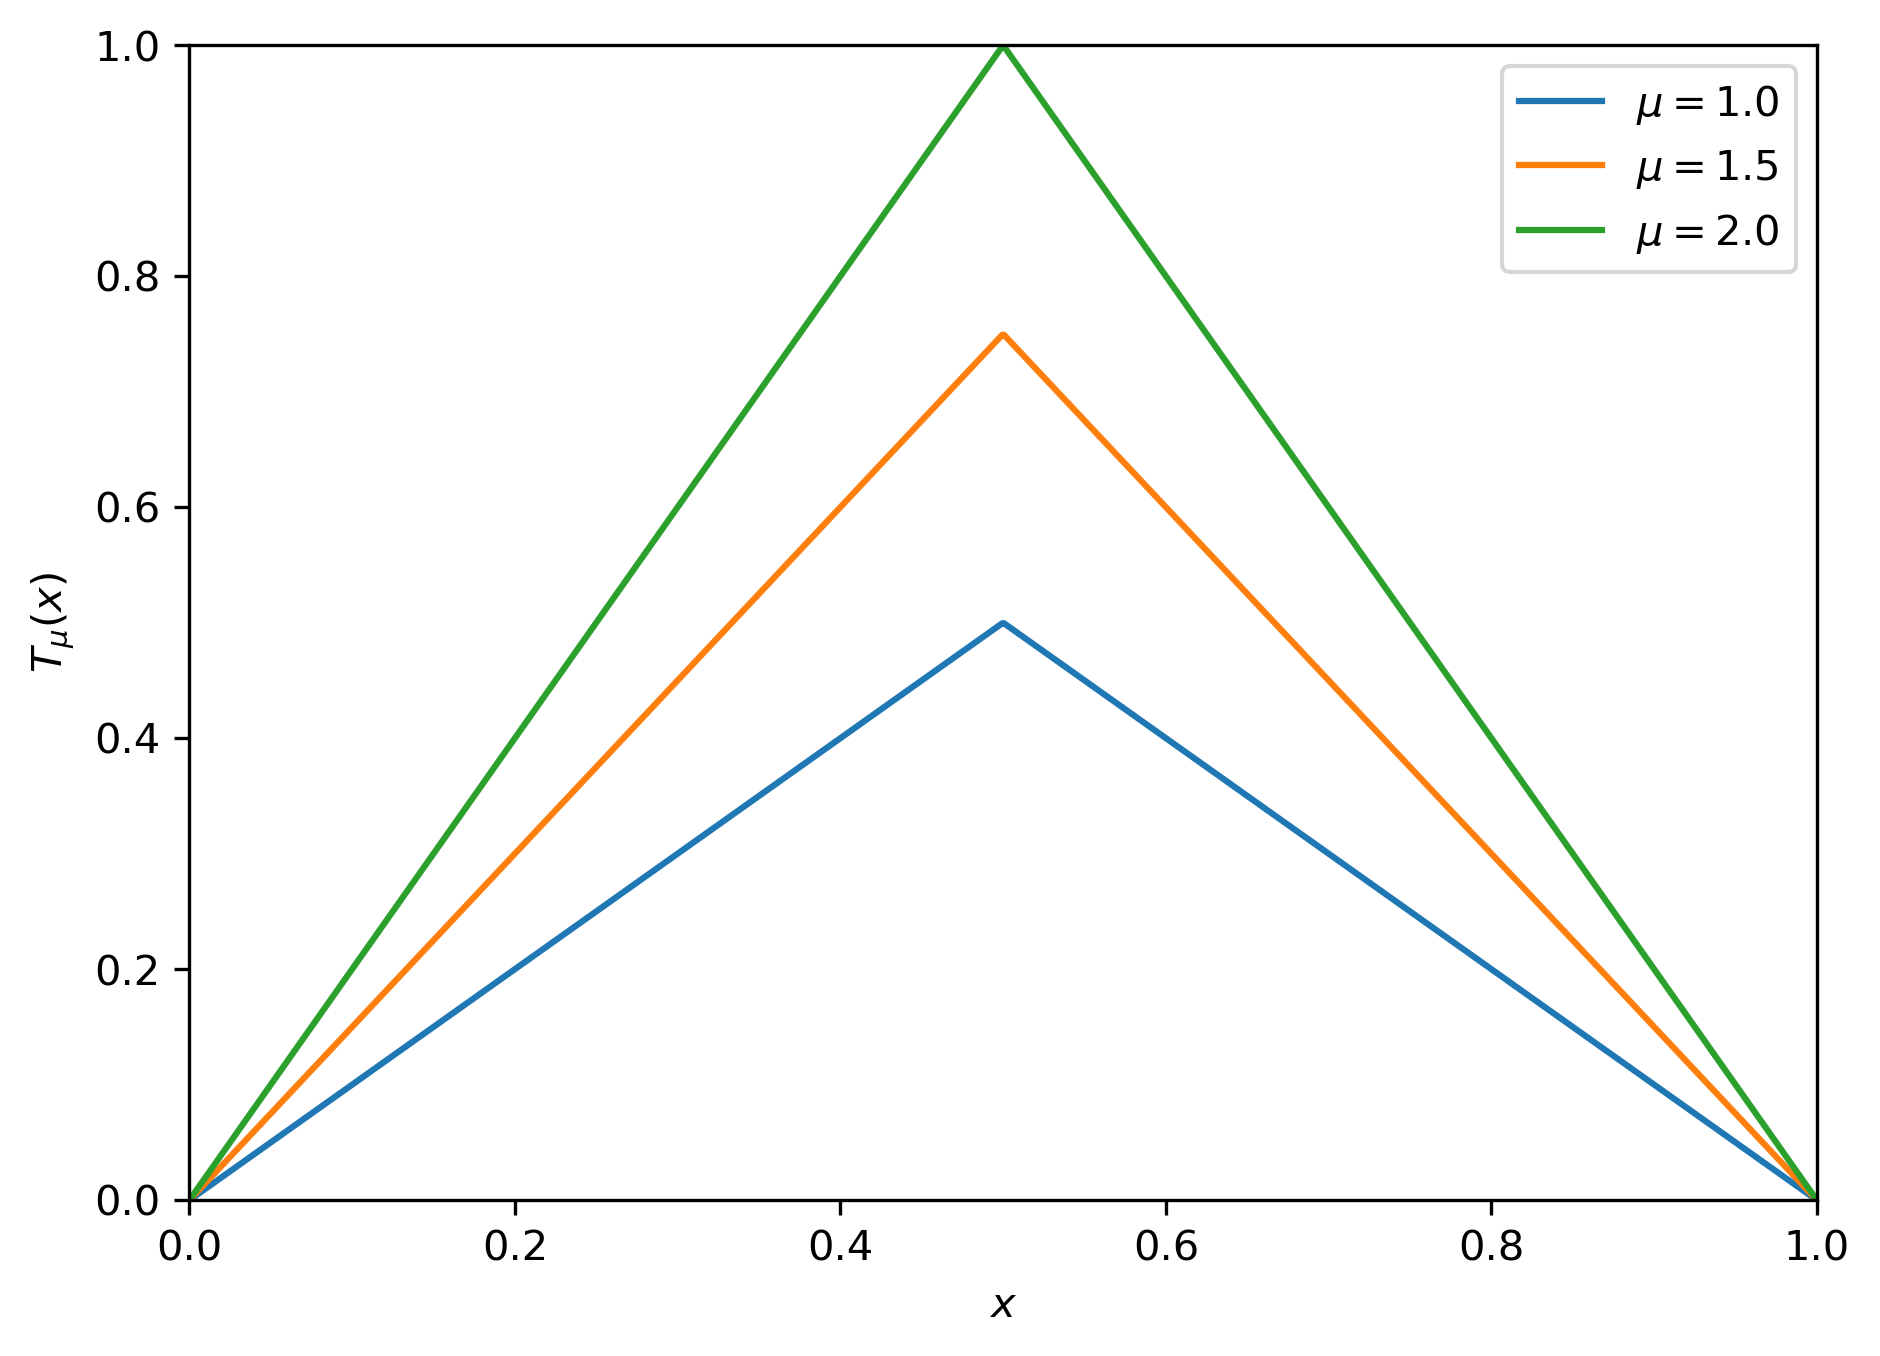
\includegraphics[height=0.8\textheight]{tent-map-fig/tent_function.png}
    \end{center}
\end{frame}

% 19
\begin{frame}{Map tent y codificaci\'on simb\'olica}
    \begin{itemize}
        \item Dividimos el intervalo:
        \[
        L=\left[0,\frac12\right],\qquad R=\left[\frac12,1\right].
        \]
        \item Cada iteraci\'on indica si la \textit{\'orbita} cae en $L$ o en $R$.
        \item As\'i se obtiene una sucesi\'on simb\'olica:
        \[
        L,R,L,L,R,\ldots
        \]
        \item Esto conecta el map tent con la din\'amica simb\'olica.
    \end{itemize}
\end{frame}

% 19b
\begin{frame}[fragile]{Diagrama de bifurcaci\'on del map tent}
    \begin{columns}[c]
        \column{0.56\textwidth}
            \centering
            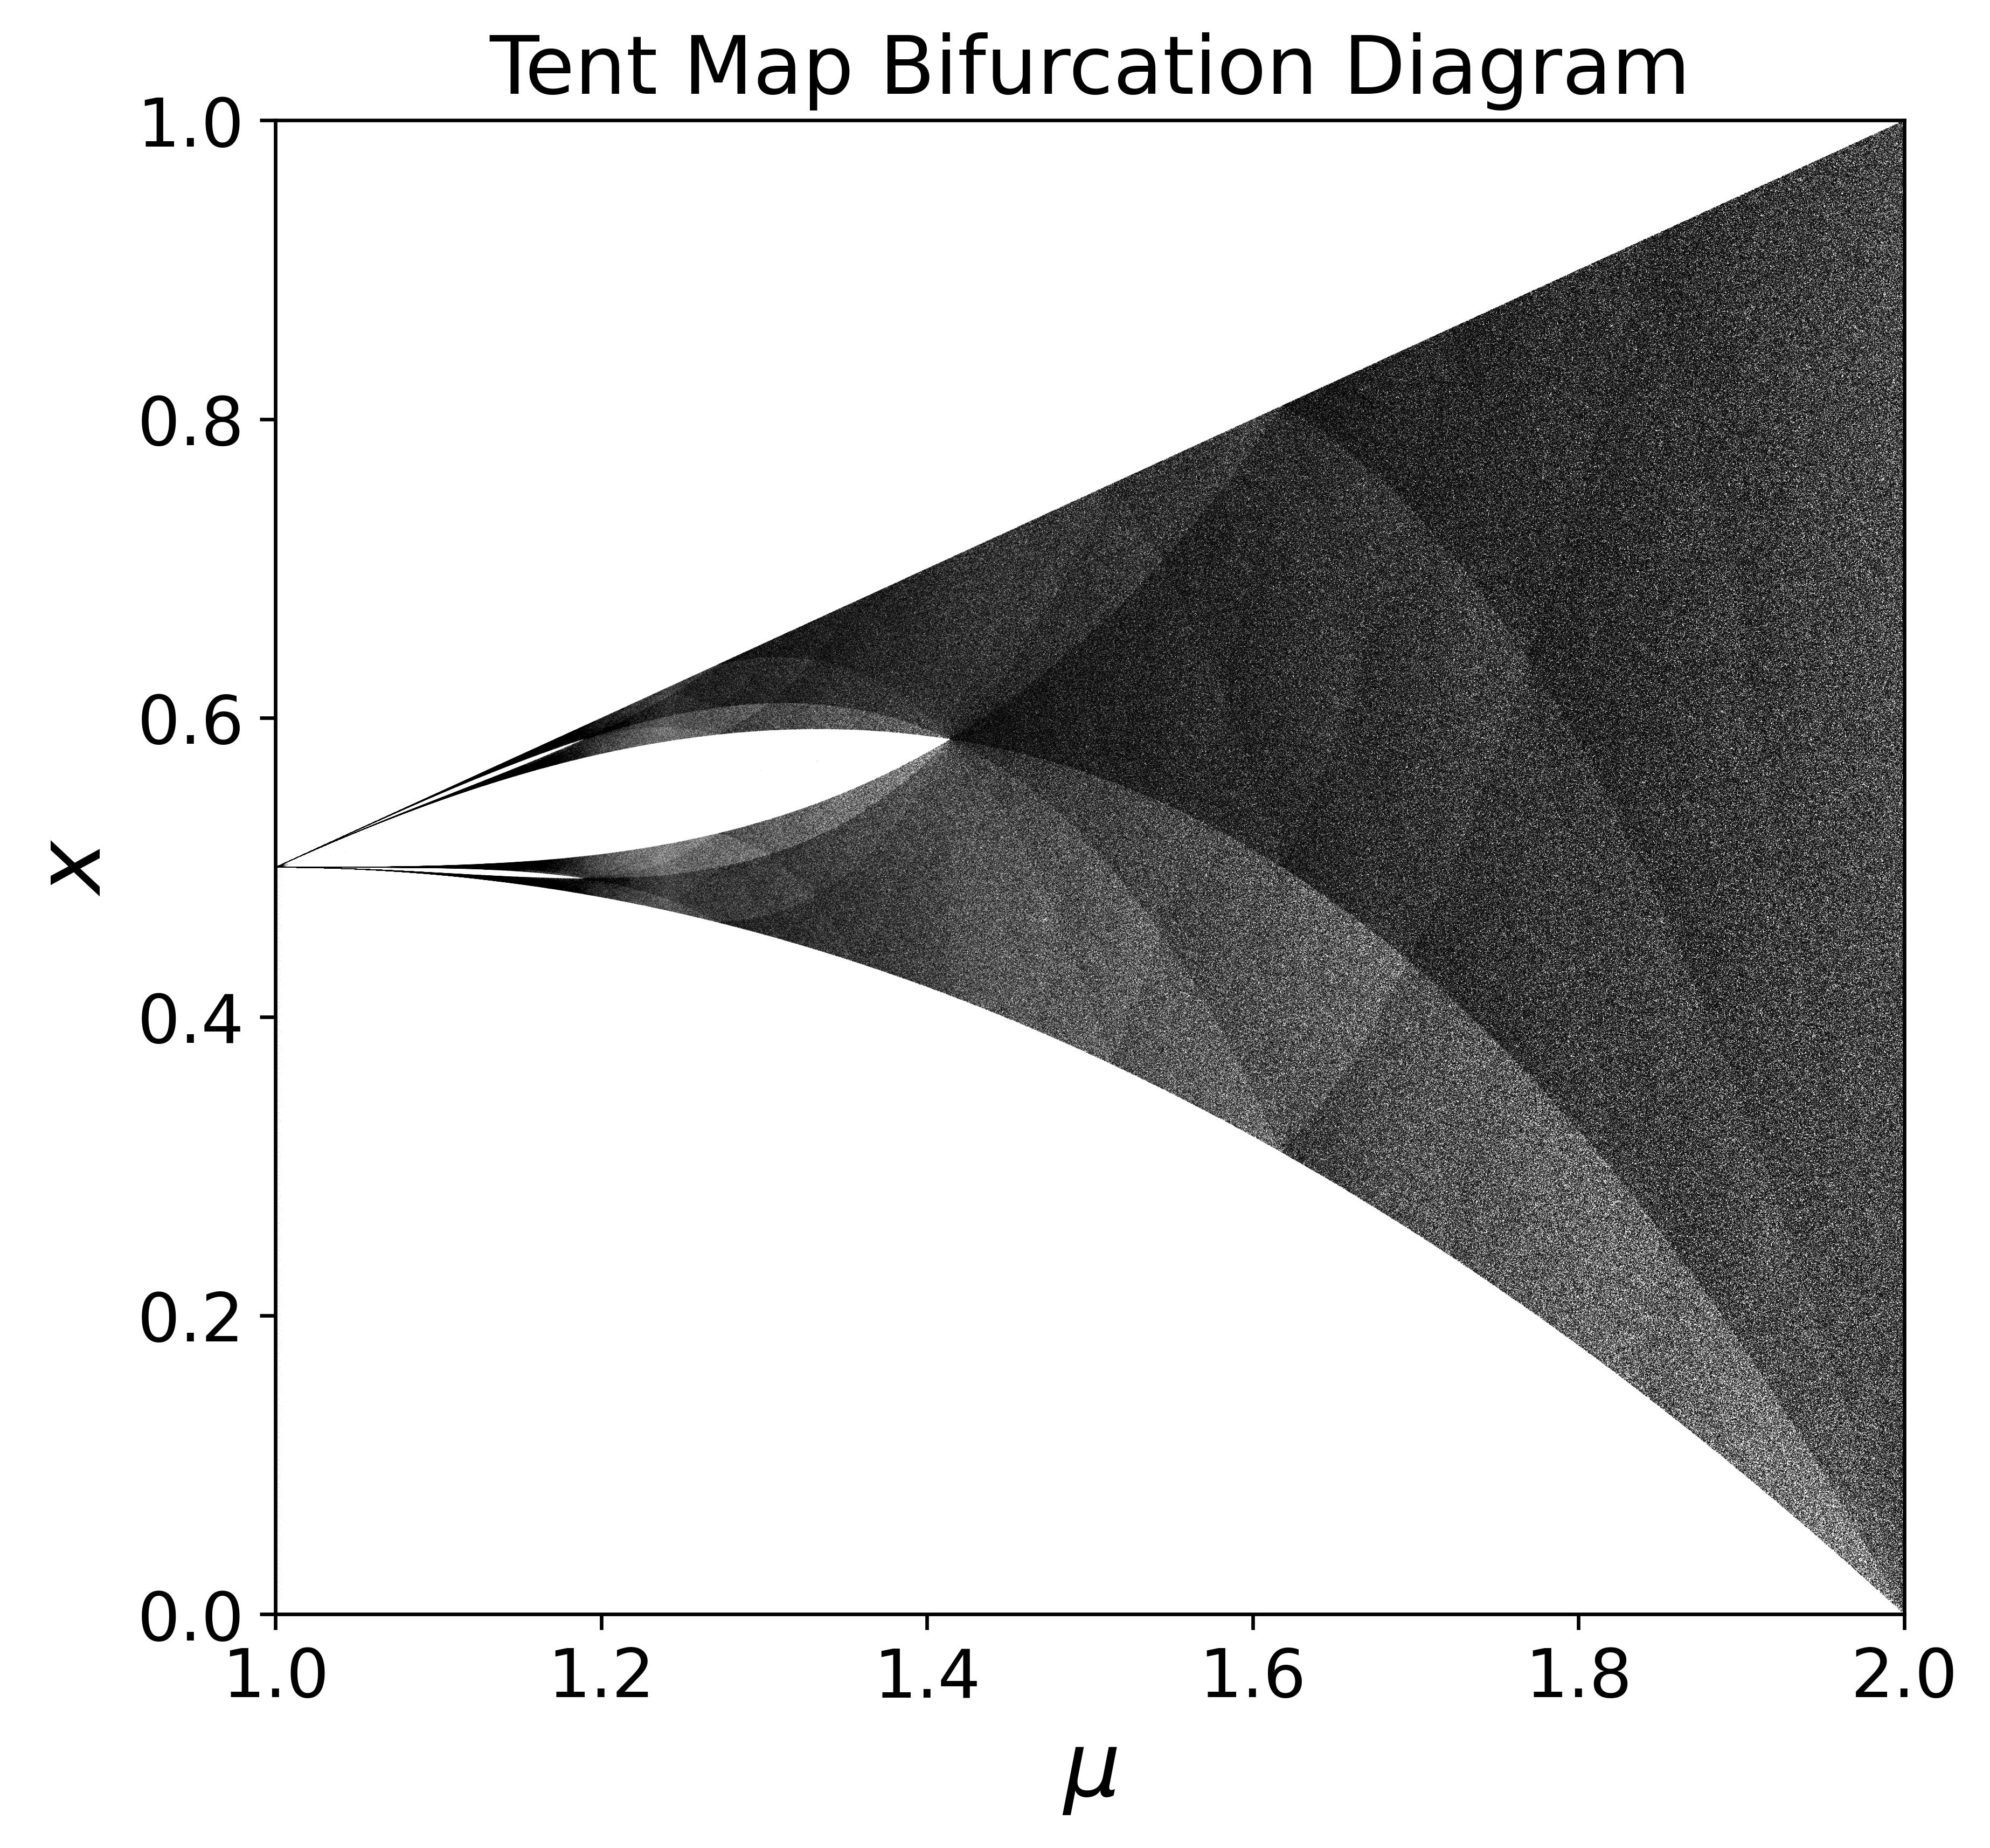
\includegraphics[width=\textwidth]{tent-map-fig/tent_map.png}
        \column{0.44\textwidth}
            \lstinputlisting[basicstyle=\ttfamily\fontsize{7.4}{8.2}\selectfont]{tent-map-fig/bifurcacion_simple.py}
    \end{columns}
\end{frame}

% 20
\begin{frame}{Cierre}
    \begin{itemize}
        \item Herramientas del curso:
        \begin{itemize}
            \item equilibrio,
            \item estabilidad,
            \item linealizaci\'on,
            \item bifurcaci\'on,
            \item adimensionalizaci\'on.
        \end{itemize}
        \item Devaney extiende esta mirada a funciones iteradas.
        \item Mensaje final:
        \[
        \text{reglas simples} \Rightarrow \text{din\'amica compleja}.
        \]
    \end{itemize}
\end{frame}

\begin{frame}{Referencias}
    \begin{thebibliography}{9}
        \bibitem{ApuntesMM1} Apuntes de Modelos Matem\'aticos I. Transcripci\'on, notas de clase y complementos con Nagle, Saff \& Snider, 7a ed. Mayo--junio de 2026.
        \bibitem{Devaney} Devaney, R. L. \emph{An Introduction to Chaotic Dynamical Systems}. Second Edition. Addison-Wesley / Westview Press.
    \end{thebibliography}
\end{frame}

\end{document}
